\newpage
\chapter{System Requirement Specification}

\section{Overall Description}
Mitsuketa is designed as a client-server application. The backend Python server handles all computationally intensive tasks---media decoding, fingerprint extraction, and database querying---while the React frontend provides a user-friendly interface for media registration and identification. Communication between the two is handled via a RESTful HTTP API.

\subsection{Block Diagram / Proposed System Setup}
The high-level system architecture of Mitsuketa is described by the following pipeline:

\begin{figure}[H]
  \centering
  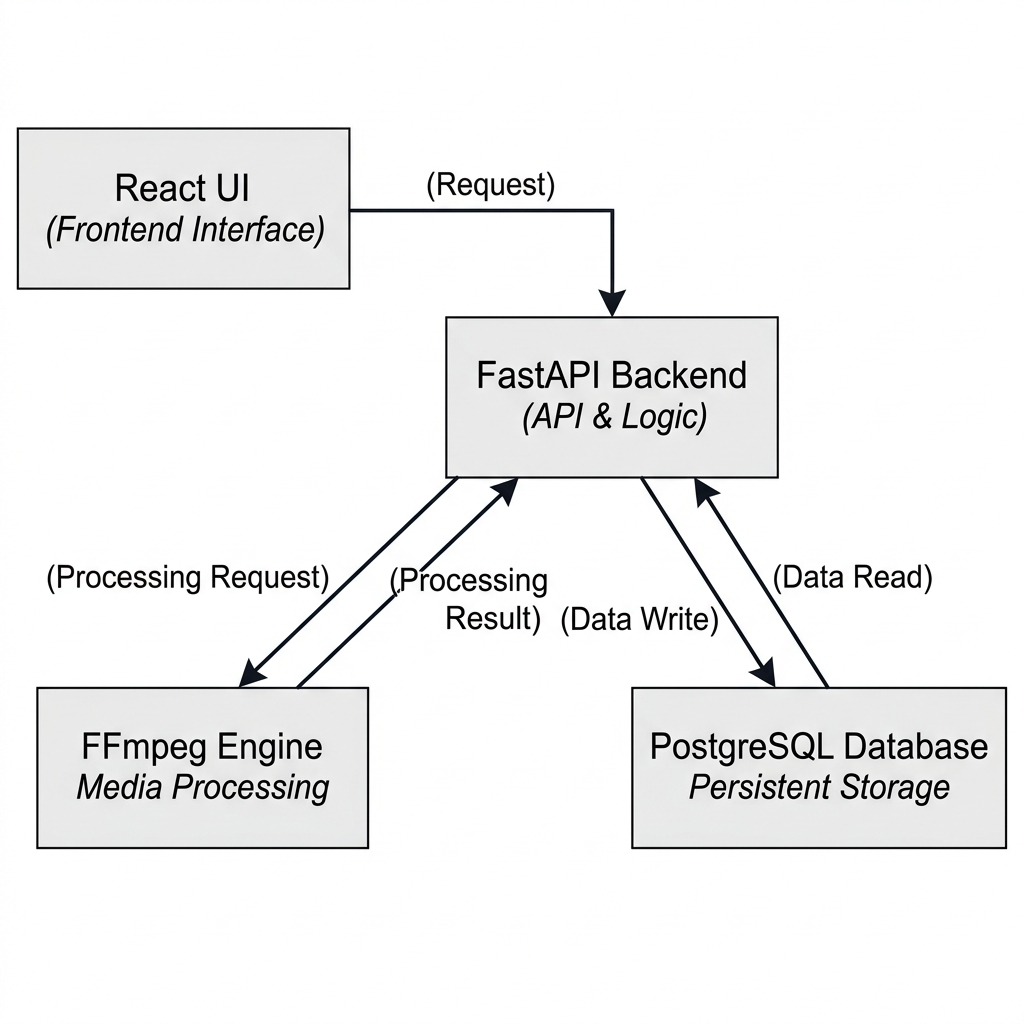
\includegraphics[width=0.6\textwidth,height=0.35\textheight,keepaspectratio]{block_diagram}
  \caption{Block Diagram of Mitsuketa -- Dual-Mode Audio-Video Fingerprinting System}\label{fig:blockdiag}
\end{figure}

\begin{itemize}
  \item \textbf{Registration Pipeline:}
    \begin{enumerate}
      \item Authorized user (Admin or Moderator) uploads a media file and a title via the React UI.
      \item Frontend sends a \texttt{POST /register} request to the FastAPI backend.
      \item FFmpeg decodes audio and extracts keyframes.
      \item Audio fingerprints (constellation map hashes) are generated by \texttt{audio\_fingerprint.py}.
      \item Video perceptual hashes (pHashes) are generated by \texttt{video\_fingerprint.py}.
      \item All fingerprints are batch-inserted into the PostgreSQL database via \texttt{database.py}.
      \item BK-Tree index is rebuilt in memory for subsequent video queries.
    \end{enumerate}
  \item \textbf{Identification Pipeline:}
    \begin{enumerate}
      \item User uploads a short query clip via the React UI.
      \item Frontend sends a \texttt{POST /identify} request.
      \item Audio fingerprints of the query are extracted.
      \item Hashes are matched against the database; temporal alignment offsets are computed.
      \item If audio confidence $>$ 35\%, a match is declared.
      \item Otherwise, video pHashes of the query are extracted and queried via the BK-Tree.
      \item A combined confidence score (0--100\%) is computed and returned to the frontend.
    \end{enumerate}
\end{itemize}

\subsection{Use Case Diagram}
The primary actors in the system are:
\begin{itemize}
  \item \textbf{User:} Interacts with the web UI to register media and submit identification queries.
  \item \textbf{FastAPI Server:} Processes registration and identification requests.
  \item \textbf{PostgreSQL Database:} Stores all user accounts, roles, media metadata, and fingerprint data persistently.
\end{itemize}

Main use cases include:
\begin{enumerate}
  \item Register a media file (Requires Moderator or Admin).
  \item Identify a query clip (Open to all authenticated users).
  \item View library of registered media.
  \item View detailed technical analysis log for a query result.
  \item Manage users and system permissions (Admin only).
\end{enumerate}

\begin{figure}[H]
  \centering
  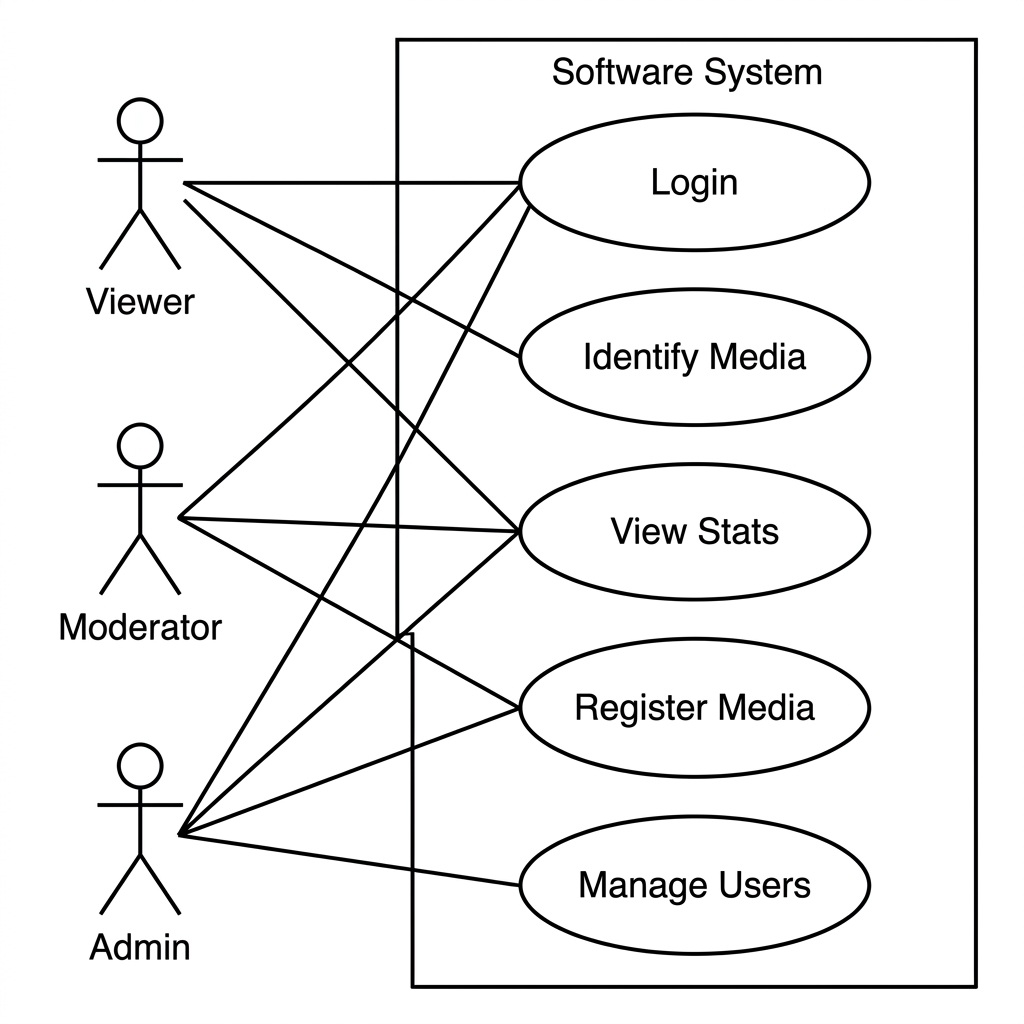
\includegraphics[width=0.6\textwidth,height=0.35\textheight,keepaspectratio]{UseCase}
  \caption{Use Case Diagram of Mitsuketa -- Video Fingerprinting System}\label{fig:usecase}
\end{figure}

\subsection{Sequence Diagram}
The identification sequence proceeds as follows:
\begin{enumerate}
  \item \textbf{User} $\rightarrow$ \textbf{React UI:} Uploads query file.
  \item \textbf{React UI} $\rightarrow$ \textbf{FastAPI:} \texttt{POST /identify} with multipart form data.
  \item \textbf{FastAPI} $\rightarrow$ \textbf{audio\_fingerprint.py:} Extract audio hashes from the query.
  \item \textbf{FastAPI} $\rightarrow$ \textbf{matcher.py:} Query database for matching audio hashes.
  \item \textbf{matcher.py} $\rightarrow$ \textbf{database.py:} Chunked read of audio fingerprint table.
  \item \textbf{matcher.py:} Compute temporal alignment offsets, produce audio confidence.
  \item \textit{If confidence insufficient:} \textbf{FastAPI} $\rightarrow$ \textbf{video\_fingerprint.py:} Extract pHashes.
  \item \textbf{FastAPI} $\rightarrow$ \textbf{matcher.py:} BK-Tree threshold query.
  \item \textbf{FastAPI} $\rightarrow$ \textbf{React UI:} Return JSON with title, confidence, and analysis log.
\end{enumerate}

\begin{figure}[H]
  \centering
  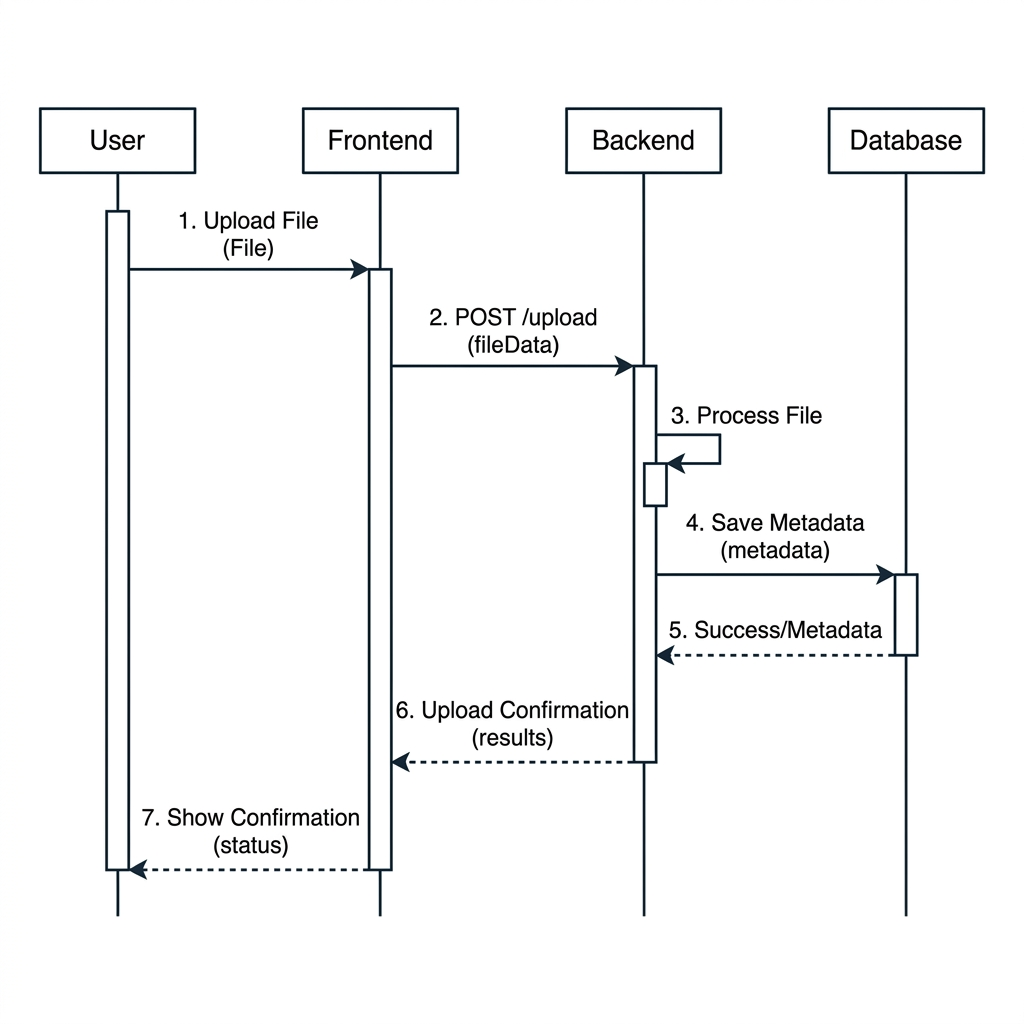
\includegraphics[width=0.6\textwidth,height=0.35\textheight,keepaspectratio]{SequenceDiagram}
  \caption{Sequence Diagram: Multimedia Content Matching Flow}\label{fig:sequence}
\end{figure}

\subsection{Entity Relationship (ER) Diagram}
The underlying PostgreSQL database schema is relational, consisting of four primary entities: \textbf{users}, \textbf{media}, \textbf{audio\_fingerprints}, and \textbf{video\_fingerprints}. This schema maps directly to the application's core functionality, enabling rapid fingerprint lookups while ensuring strict role-based data integrity.

\begin{figure}[H]
  \centering
  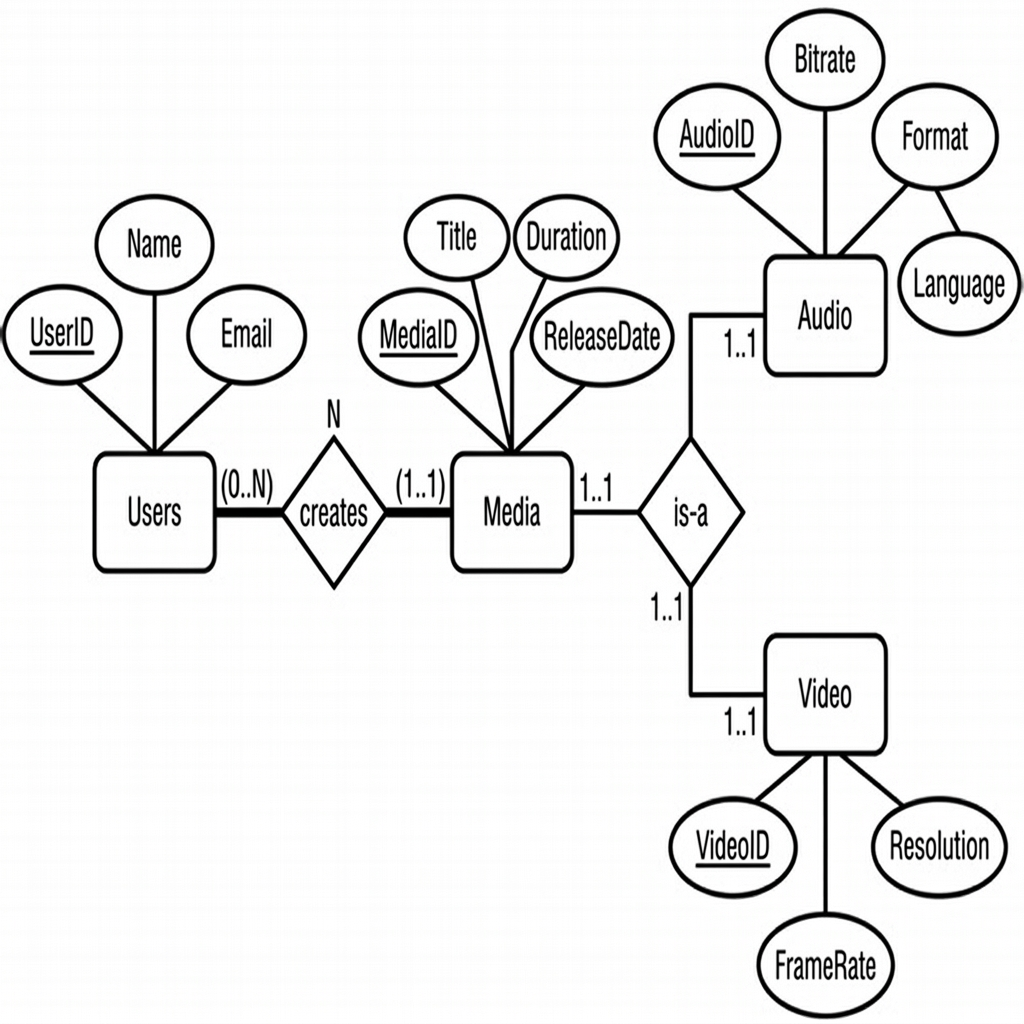
\includegraphics[width=0.6\textwidth,height=0.35\textheight,keepaspectratio]{ERDiagram}
  \caption{Entity Relationship Diagram mapping the PostgreSQL Database Structure}\label{fig:erdiagram}
\end{figure}

\subsection{Related Mathematical Modelling}
The confidence score $C$ is computed as a weighted combination:
\begin{equation}
  C = \begin{cases}
    C_{\text{audio}} & \text{if } C_{\text{audio}} > 35\% \\
    C_{\text{video}} & \text{otherwise}
  \end{cases}
\end{equation}
where:
\begin{equation}
  C_{\text{audio}} = \frac{N_{\text{aligned}}}{N_{\text{query}}} \times 100\%
\end{equation}
\begin{equation}
  C_{\text{video}} = \left(1 - \frac{d_H}{64}\right) \times 100\%
\end{equation}
with $N_{\text{aligned}}$ being the number of temporally aligned hash matches, $N_{\text{query}}$ the total hashes from the query clip, and $d_H$ the Hamming distance between matched pHash pairs.

\subsection{Hardware and Software Requirements}
(Refer to Section 3.4 for a detailed listing of hardware and software requirements.)

\section{Project Planning}
\begin{table}[h!]
\centering
\caption{Project Timeline and Milestones (August 2025 -- April 2026)}
\label{tab:planning}
\begin{tabular}{p{0.5cm} p{5.5cm} p{3cm} p{3cm}}
\noalign{\hrule height 0.5mm}
\textbf{No.} & \textbf{Task} & \textbf{Start} & \textbf{End} \\
\hline
1 & Literature review and problem formulation    & 1 Aug 2025  & 31 Aug 2025  \\
2 & Audio fingerprinting engine development       & 1 Sep 2025  & 30 Sep 2025  \\
3 & Database design and SQLite integration        & 1 Oct 2025  & 20 Oct 2025  \\
4 & Video fingerprinting and BK-Tree implementation & 21 Oct 2025 & 15 Nov 2025  \\
5 & FastAPI backend and REST API development      & 16 Nov 2025 & 30 Nov 2025  \\
6 & React frontend design and integration         & 1 Dec 2025  & 31 Dec 2025  \\
7 & Testing, debugging, and performance evaluation & 1 Jan 2026  & 28 Feb 2026  \\
8 & Report writing and final submission            & 1 Mar 2026  & 1 Apr 2026   \\
\noalign{\hrule height 0.5mm}
\end{tabular}
\end{table}

\vspace{10mm}
\hrule